\subsection{单时段证券模型}

某股票现价为100美元,在一年后股价可以是90美元或120美元,概率并未给定,即期利率(实际利率)是5\%。一年之后到期执行价为105美元的股票期权的公平价格是多少?

\subsubsection{构造无风险对冲组合方法}

若期权的价格为 $V$,股票的价格为 $S$,构造如下的资产组合: 持有 $a$ 股期权和 $b$ 股股票,若 $a<0$ 或 $b<0$ 表示空头 。则 $t=0$ 时资产组合的价值
\[
\Pi_0=aV+bS
\]
这里 $a,b$ 是未知的。当 $t=1$ 时:
\[
\Pi_1=\begin{cases}
    (120-105)a+105b & S_1=120\\
    a\cdot 0+90b & S_1=90
\end{cases}
\]
让 $\Pi_1$ 不取决于股价涨跌
\[
    (120-105)a+105b=a\cdot 0+90b
\]
解得
\[
a=-2b
\]
令 $b=1$,则 $a=-2$
\[
\Pi_0=-2V+1\times 100
\]
\[
\Pi_1=-2\times(120-105)+1\times 120=-2\times 0+1\times 90
\]
由于组合 $\Pi$ 是无风险的,根据无套利原理,其收益率应等于即期利率 5\%,因此 $1.05\Pi_0=\Pi_1$,即
\[
1.05(100-2V)=90
\]
解得 $V=7.14286$

\vspace{1em}

\begin{minipage}{0.5\textwidth}
    \begin{center}
        \begin{forest}
            for tree={grow'=east, l sep=30pt, s sep=15pt, inner sep=2pt}
            [{$S_0$}
                [{$S_u$}, edge label={node[midway,above]{$p$}}]
                [{$S_d$}, edge label={node[midway,below]{$1-p$}}]
            ]
        \end{forest}
    \end{center}
\end{minipage}
\hfill
\begin{minipage}{0.5\textwidth}
    \begin{center}
        \begin{forest}
            for tree={grow'=east, l sep=30pt, s sep=15pt, inner sep=2pt}
            [{$V$}
                [{$U$}, edge label={node[midway,above]{$p$}}]
                [{$D$}, edge label={node[midway,below]{$1-p$}}]
            ]
        \end{forest}
    \end{center}
\end{minipage}

\vspace{1em}

左图为股价二叉树,右图为衍生产品价格二叉树

\begin{definition}[无风险对冲组合]
构造资产组合:1份衍生产品多头和 $\alpha$ 份股票空头。资产组合的初始价值为:
\[
\Pi_0=V-\alpha S_0
\]
选择 $\alpha$,使得资产组合的价值与股票的最终价值无关,称该组合为无风险对冲组合
\end{definition}

\[
\Pi_1=\begin{cases}
    \Pi_1^u=U-\alpha S_u & \text{股价上升}\\
    \Pi_1^d=D-\alpha S_d & \text{股价下降}
\end{cases}
\]
\[
U-\alpha S_u=D-\alpha S_d
\]
\[
\Rightarrow \alpha=\frac{U-D}{S_u-S_d}=\frac{\Delta V}{\Delta S}
\]
资产组合的初始价值:$V-\alpha S_0$

资产组合的最终价值:$U-\alpha S_u$

若无风险利率为 $r$(该时间段实际利率),则
\[
    V-\alpha S_0=\frac{U-\alpha S_u}{1+r}
\]
于是得到衍生产品的定价公式
\[
    V=\alpha S_0+\frac{U-\alpha S_u}{1+r}
\]

\subsubsection{资产组合复制方法}

\begin{definition}[复制]
构造资产组合:包含 $a$ 单位的股票和 $b$ 单位的现金,无风险资产利率为 $r$,则在 $t=0$ 时:
\[
V_0=aS_0+b
\]
若在 $\forall t,\forall \omega\in \Omega$ 下,该组合价值都与衍生品 $C$ 价值相同,则称该资产组合为衍生品 $C$ 的一个复制
\end{definition}

在 $t=1$ 时
\[
V_1=\begin{cases}
    V_1^u=aS_u+b(1+r)\\
    V_1^d=aS_d+b(1+r)
\end{cases}
\]
令
\[
\begin{cases}
    aS_u+b(1+r)=U\\
    aS_d+b(1+r)=D
\end{cases}
\]
于是资产组合的价值和衍生证券的价值一致,该资产组合复制了衍生证券$V$。

解得
\[
\begin{aligned}
    a&=\frac{U-D}{S_u-S_d}\\
    b&=(U-\frac{U-D}{S_u-S_d}S_u)/(1+r)
\end{aligned}
\]
\[
\begin{aligned}
    V_0&=aS_0+b\\
    &=\frac{U-D}{S_u-S_d}S_0+(U-\frac{U-D}{S_u-S_d}S_u)/(1+r)
\end{aligned}
\]
将 $U$ 和 $D$ 分开得
\[
\begin{aligned}
    V_0&=\left(\frac{S_0}{S_u-S_d}+\frac{1}{1+r}-\frac{S_u}{S_u-S_d}\cdot \frac{1}{1+r}\right)U-\left(-\frac{S_0}{S_u-S_d}+\frac{S_u}{S_u-S_d}\cdot \frac{1}{1+r}\right)D\\
    &=\frac{1}{1+r}\left(\frac{(1+r)S_0}{S_u-S_d}-\frac{S_d}{S_u-S_d}\right)U+\frac{1}{1+r}\left(\frac{S_u}{S_u-S_d}-\frac{(1+r)S_0}{S_u-S_d}\right)D\\
    &=\frac{1}{1+r}[qU+(1-q)D]
\end{aligned}
\]
其中
\[
\begin{aligned}
    q&=\frac{(1+r)S_0}{S_u-S_d}-\frac{S_d}{S_u-S_d}\\
    1-q&=\frac{S_u}{S_u-S_d}-\frac{(1+r)S_0}{S_u-S_d}
\end{aligned}
\]
$q$ 的意义是什么?

由无套利性可知
\[
0<q<1
\]
由 $q$ 的表达式可知
\[
S_0=\frac{1}{1+r}[qS_u+(1-q)S_d]
\]
若令股票上涨、下跌的概率分别为 $q,1-q$,记此概率测度为 $\QQ$,则
\[
S_0=\frac{1}{1+r}\EE_Q(S_1)
\]
其中 $S_1$ 为股票在 $t=1$ 时刻的价值

进一步
\[
    V=\frac{1}{1+r}\EE_Q(V_1)=\EE_Q\left[\frac{V_1}{1+r} \right]
\]
其中 $V_1$ 为期权在 $t=1$ 时刻的价值

问题:若证券种类更多,市场状态也更多的情况下,上述结论是否成立?

\subsubsection{多个市场状态下投资组合定价}

$M$ 种风险资产价格过程 $S_1(t),S_2(t),\cdots,S_M(t), t=0,1$。在$t=1$ 时刻有 $K$ 种可能的市场状态 $\Omega=\{\omega_1,\omega_2,\cdots,\omega_K\}$

在 $t=1$ 时刻风险资产的可能值表示为一个非负 $K\times M$ 矩阵,被称为 Payoff Matrix
\[
S(1;\Omega)=\begin{pmatrix}
    S_1(1;\omega_1) & S_2(1;\omega_1) & \cdots & S_M(1;\omega_1)\\
    S_1(1;\omega_2) & S_2(1;\omega_2) & \cdots & S_M(1;\omega_2)\\
    \vdots & \vdots & \cdots & \vdots\\
    S_1(1;\omega_K) & S_2(1;\omega_K) & \cdots & S_M(1;\omega_K)
\end{pmatrix}
\]
每个列向量表示每个资产在所有市场状态下的价格,记为
\begin{equation}
S_m(t)=(S_m(t;\omega_i))_{i=1:K}=\begin{pmatrix}
    S_m(t;\omega_1)\\
    S_m(t;\omega_2)\\
    \vdots\\
    S_m(t;\omega_K)
\end{pmatrix},\quad t\geq 1
\label{eq:Smt}
\end{equation}
当 $t=0$ 时,资产 $m$ 的价值是确定的,因此 $S_m(0)$ 不是一个向量而是一个数值

用列向量的形式表示 $S(1;\Omega)$ 矩阵
\begin{equation}
S(1;\Omega)=(S_1(1)|\cdots |S_M(1))=\text{col}(S_m(1))_{m=1:K}
\label{eq:vanilla_payoff}
\end{equation}
考虑无风险证券 $S_0(t),t=0,1$
\[
\begin{aligned}
    S_0(0)&=S_0(0;\omega)=1\\
    S_0(1)&=S_0(1;\omega)=1+r, \quad \forall \omega\in \Omega
\end{aligned}
\]
结合\eqref{eq:Smt}, 风险资产贴现价格过程
\begin{equation}
S_m^*(t)=\frac{S_m(t)}{S_0(t)}=\begin{pmatrix}
    S_m(t;\omega_1)/S_0(t)\\
    S_m(t;\omega_2)/S_0(t)\\
    \vdots\\
    S_m(t;\omega_K)/S_0(t)
\end{pmatrix},\quad t\geq 0,\quad m=1,2,\cdots,M
\label{eq:discount_vector}
\end{equation}
其中 $S_m(t)$ 为 $K\times 1$ 的列向量,$S_0(t)$ 是一个由 $t$ 决定的数值,因此 $S_m^*(t)$ 也为 $K\times 1$ 的列向量

写成矩阵形式
\[
S^*(1;\Omega)=\begin{pmatrix}
    S_1^*(1;\omega_1) & S_2^*(1;\omega_1) & \cdots & S_M^*(1;\omega_1)\\
    S_1^*(1;\omega_2) & S_2^*(1;\omega_2) & \cdots & S_M^*(1;\omega_2)\\
    \vdots & \vdots & \cdots & \vdots\\
    S_1^*(1;\omega_K) & S_2^*(1;\omega_K) & \cdots & S_M^*(1;\omega_K)
\end{pmatrix}
\]
即
\begin{equation}
S^*(1;\Omega)=(S_1^*(1)|\cdots |S_M^*(1))=\text{col}(S_m^*(1))_{m=1:K}
\label{eq:discount_payoff}
\end{equation}
所有资产在 $t=1$ 时刻的价格矩阵被称为扩展形式的 Payoff Matrix,如下所示
\[
\hat{S}(1;\Omega)=\begin{pmatrix}
    1+r & S_1(1;\omega_1) & S_2(1;\omega_1) & \cdots & S_M(1;\omega_1)\\
    1+r & S_1(1;\omega_2) & S_2(1;\omega_2) & \cdots & S_M(1;\omega_2)\\
    \vdots & \vdots & \vdots & \cdots & \vdots\\
    1+r & S_1(1;\omega_K) & S_2(1;\omega_K) & \cdots & S_M(1;\omega_K)
\end{pmatrix}
\]
第一列是无风险资产在 $t=1$ 时刻的价值,是一个 $K\times 1$ 的列向量。一般形式为
\begin{equation}
S_0(t)=(S_0(t;\omega_i))_{i=1:K}
\label{eq:S0t}
\end{equation}
结合\eqref{eq:Smt},则
\begin{equation}
\hat{S}(1;\Omega)=\text{col}(S_m(1))_{m=0:M}
\label{eq:extend_payoff}
\end{equation}
所有资产在 $t=0$ 时刻的价格向量为
\begin{equation}
\hat{S}(0)=(1,S_1(0),S_2(0),\cdots,S_M(0))^T
\label{eq:extend_S0_vec}
\end{equation}
所有资产在 $t=1$ 时刻的贴现价格矩阵为
\[
\hat{S}^*(1;\Omega)=\begin{pmatrix}
    1 & S_1^*(1;\omega_1) & S_2^*(1;\omega_1) & \cdots & S_M^*(1;\omega_1)\\
    1 & S_1^*(1;\omega_2) & S_2^*(1;\omega_2) & \cdots & S_M^*(1;\omega_2)\\
    \vdots & \vdots & \vdots & \cdots & \vdots\\
    1 & S_1^*(1;\omega_K) & S_2^*(1;\omega_K) & \cdots & S_M^*(1;\omega_K)
\end{pmatrix}
\]
即
\begin{equation}
\hat{S}^*(1;\Omega)=(S_0^*(1)|S_1^*(1)|\cdots |S_M^*(1))=\text{col}(S_m^*(1))_{m=0:M}
\label{eq:extend_discount_payoff}
\end{equation}
其中 $S_m^*(t)$ 为 $K\times 1$ 的列向量\eqref{eq:discount_vector},并且 $S_0^*(t)=(1,\cdots,1)^T$.

所有资产在 $t=0$ 时刻的贴现价格向量为
\begin{equation}
\hat{S}^*(0)=(1,S_1^*(0),S_2^*(0),\cdots,S_M^*(0))^T
\label{eq:discount_S0_vec}
\end{equation}
故 $\hat{S}^*(0)=\hat{S}(0)$

\subsubsection{套利机会}

在 $t=0$ 时刻的交易策略为 $\{h_m,m=0,1,\cdots,M\}$,其中 $h_m$ 为第 $m$ 个资产的持有份额。记所有资产权重向量为 $\hat{h}=(h_i)_{i=0:M}$ 此投资组合价值过程为
\begin{equation}
V_t=h_0S_0(t)+\sum_{m=1}^Mh_mS_m(t)
\label{eq:portfolio_value}
\end{equation}
其中 $S_m(t), S_0(t)$ 均为 $K\times 1$ 的价格向量,见\eqref{eq:Smt}, \eqref{eq:S0t}。因此 $V_t$ 也为 $K\times 1$ 的向量。

将\eqref{eq:portfolio_value}写成矩阵形式,即
\begin{equation}
V_t=\hat{S}(1;\Omega)\hat{h}
\label{eq:portfolio_value_matrix_form}
\end{equation}
其中 $\hat{S}(1;\Omega)$ 为扩展形式的 Payoff Matrix\eqref{eq:extend_payoff}。
Elementwise的表示\eqref{eq:portfolio_value}在计算中更常用,但矩阵形式\eqref{eq:portfolio_value_matrix_form}能更好的帮助我们理解。

投资组合收益
\begin{equation}
G\overset{\Delta}{=}V_1-V_0=h_0r\cdot \textbf{1}_K+\sum_{m=1}^M h_m\cdot \Delta S_m
\label{eq:growth}
\end{equation}

其中 $\textbf{1}_K$ 为长度为 $K$ 的全1列向量,且
\begin{equation}
\Delta S_m\overset{\Delta}{=} S_m(1)-S_m(0)=\begin{pmatrix}
    S_m(1;\omega_1)-S_m(0)\\
    S_m(1;\omega_2)-S_m(0)\\
    \vdots\\
    S_m(1;\omega_K)-S_m(0)
\end{pmatrix}
\end{equation}

投资组合贴现价值过程
\begin{equation}
V_t^*\overset{\Delta}{=}h_0\cdot \textbf{1}_K+\sum_{m=1}^M h_m S_m^*(t)
\label{eq:discount_portfolio_value}
\end{equation}
其中 $\textbf{1}_K$ 为长度为 $K$ 的全1列向量,$S_m^*(t)$ 为 $K\times 1$ 的列向量\eqref{eq:discount_vector}。将\eqref{eq:discount_portfolio_value}写成矩阵形式,即
\begin{equation}
V_t^*=\hat{S}^*(1;\Omega)\hat{h}
\label{eq:discount_portfolio_value_matrix_form}
\end{equation}
其中 $\hat{S}^*(1;\Omega)$ 为扩展形式的贴现Payoff Matrix\eqref{eq:extend_discount_payoff}.

投资组合贴现收益为
\begin{equation}
G^*\overset{\Delta}{=}V_1^*-V_0^*=\sum_{m=1}^M h_m\cdot \Delta S_m^*
\label{eq:discount_growth}
\end{equation}
其中
\begin{equation}
\Delta S_m^*\overset{\Delta}{=} S_m^*(1)-S_m^*(0)=\begin{pmatrix}
    S_m^*(1;\omega_1)-S_m^*(0)\\
    S_m^*(1;\omega_2)-S_m^*(0)\\
    \vdots\\
    S_m^*(1;\omega_K)-S_m^*(0)
\end{pmatrix}
\label{eq:delta_Sm}
\end{equation}
可以将每个风险资产的 $\Delta S_m^*$ 合并写成矩阵形式
\begin{equation}
\Delta S^*=(\Delta S_1^* | \cdots | \Delta S_M^*)=\text{col}(\Delta S_m^*)_{m=1:M}\in \RR^{K\times M}
\label{eq:delta_Sm_matrix}
\end{equation}

\begin{definition}[套利机会]
    某个交易策略被称为套利机会,如果
    \begin{enumerate}
        \item $V_0^*=0$
        \item $V_1^*(\omega)\geq 0, \forall \omega\in \Omega$ 且 $\EE(V_1^*)>0$
    \end{enumerate}
    其中 $\EE$ 为在实际概率测度 $\PP$ 下的期望
\end{definition}

注:(2)等价于 $V_1^*(\omega)\geq 0, \forall \omega\in \Omega$ 且 $\PP(V_1^*>0)>0$

不妨设 $\PP(\omega)>0,\forall \omega\in \Omega$,则(2)又等价于 $V_1^*(\omega)\geq 0, \forall \omega\in \Omega$ 且不等号对于某个 $\omega\in \Omega$ 严格成立

\begin{lemma}[套利机会等价条件]
    存在套利机会

    $\Leftrightarrow$ 存在交易策略 $\hat{h}=(h_0,h_1,\cdots,h_m)^T$,使得 $\hat{S}^*(0)\hat{h}=0, \hat{S}^*(1;\Omega)\hat{h}\geq 0$ 且不等号对某个 $\omega\in \Omega$ 严格成立。其中 $\hat{S}^*(0),\hat{S}^*(1;\Omega)$ 分别为\eqref{eq:discount_S0_vec}, \eqref{eq:extend_discount_payoff}.

    $\Leftrightarrow$ 存在交易策略 $\{h_m,m=0,1,\cdots,M\}$,使得 $G^*(\omega)\geq 0, \forall \omega\in \Omega$ 且不等号对某个 $\omega\in \Omega$ 严格成立。其中 $G^*$ 为\eqref{eq:discount_growth}.

    $\Leftrightarrow$ 存在交易策略 $h=(h_1,\cdots,h_m)^T$ 使得 $(\Delta S^*)h\geq 0$ 且在上述向量不等式中,不等号至少对某个元素严格成立。其中 $\Delta S^*$ 为 \eqref{eq:delta_Sm_matrix}.
\end{lemma}

证明:

\subsubsection{风险中性测度}

\begin{definition}[风险中性概率测度]\label{def:risk-neutral}
    $\Omega$ 上的概率测度 $\QQ$ 被称为风险中性概率测度,如果
    \begin{enumerate}
        \item $\QQ(\omega)>0,\forall \omega\in \Omega$
        \item $\EE_Q[\Delta S_m^*]=0,\forall m=1,2,\cdots,M$,即
        \[
        S_m^*(0)=\EE_Q[S_m^*(1)]
        \]
        其中 $\EE_Q$ 表示在测度 $\QQ$ 下的期望
    \end{enumerate}
\end{definition}

记风险中性测度 $\Pi=(\QQ(\omega_1), \QQ(\omega_2), \cdots,\QQ(\omega_K))$,则上述条件(2)的等价条件为
\[
\begin{aligned}
    \EE_Q[\Delta S_m^*]=0 &\Leftrightarrow \Pi\cdot(\Delta S_m^*)=0,\forall m=1,2,\cdots,M\\
    &\Leftrightarrow \Pi\cdot(\Delta S^*)=0\\
    &\Leftrightarrow \text{对任意交易策略 } V_0^*=\EE_Q(V_1^*),\text{亦即} \EE_Q(G^*)=0
\end{aligned}
\]
其中 $\Delta S_m^*, \Delta S^*$ 分别为 \eqref{eq:delta_Sm}, \eqref{eq:delta_Sm_matrix}。分析如下:
\[
\begin{aligned}
    \EE_Q[\Delta S_m^*]=0 &\Leftrightarrow \Pi\cdot[S^*(1;\Omega)]=S^*(0), \sum_{i=1}^K \QQ(\omega_i)=1, \QQ(\omega_i)\geq 0,\forall i=1,\cdots,K\\
    &\Leftrightarrow \Pi\cdot[\hat{S}^*(1;\Omega)]=\hat{S}^*(0), \QQ(\omega_i)\geq 0,\forall i=1,\cdots,K\\
    &\Leftrightarrow \Pi\cdot(\Delta S^*)=0, \sum_{i=1}^K \QQ(\omega_i)=1, \QQ(\omega_i)\geq 0,\forall i=1,\cdots,K
\end{aligned}
\]
应用:对任意投资组合 $V$,其由 $M+1$ 种资产构成,权重为 $(h_0,h_1,\cdots,h_M)$。在 $t=1$ 时刻有 $K$ 种可能的市场状态,对应各种资产的贴现价值表示为 $\hat{S}^*(1;\Omega)=$
\[
\begin{aligned}
    \EE_Q(V_1^*)=\sum_{i=1}^K V_1^*(\omega_i)\QQ(\omega_i)&=\sum_{i=1}^K\sum_{j=0}^M h_j\cdot S^*_j(1;\omega_i)\cdot \QQ(\omega_i)\\
    &=\sum_{j=0}^M\sum_{i=1}^K h_j\cdot S^*_j(1;\omega_i)\cdot \QQ(\omega_i)\\
    &=\sum_{j=0}^M h_j \underbrace{\sum_{i=1}^K S^*_j(1;\omega_i)\cdot \QQ(\omega_i)}_{\text{第}j\text{种资产的贴现价值期望}}\\
    &=\sum_{j=0}^M h_j\cdot \EE_Q(S_j^*(1))\\
    &=\sum_{j=0}^M h_j\cdot S^*_j(0)\quad [\text{风险中性定义\eqref{def:risk-neutral}}]\\
    &=\sum_{j=0}^M h_j\cdot S_j(0)=V_0=V^*(0)
\end{aligned}
\]

\subsubsection{凸集分离定理}

向量投影:$f=(f_1,f_2,\cdots,f_n)\in\RR^n, x=(x_1,\cdots,x_n)\in \RR^n$

向量 $x$ 在 $f$ 上的投影:(夹角为 $\alpha$)

\vspace{1em}

\begin{minipage}{0.5\textwidth}
    \begin{figure}[H]
        \centering
        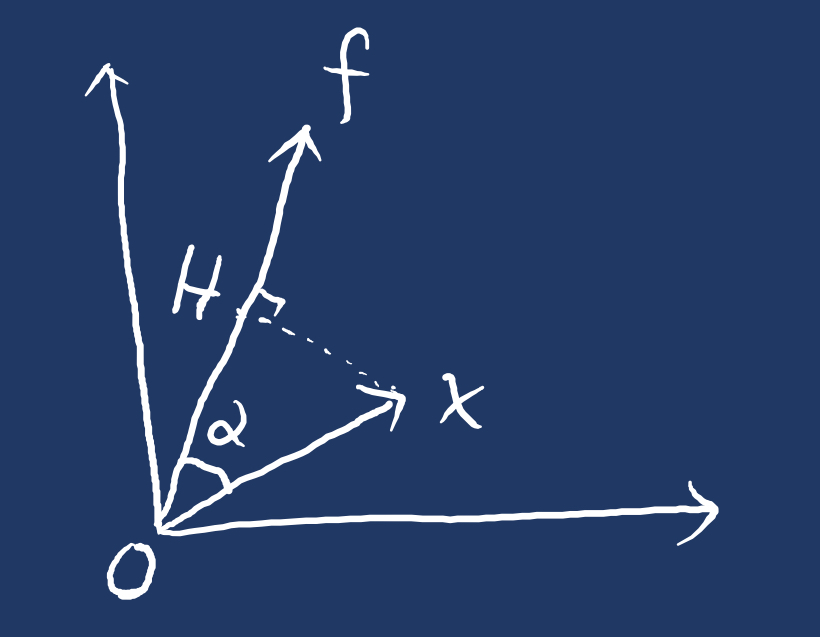
\includegraphics[width=0.6\textwidth]{figures/向量投影.jpeg} % 替换为你的图片文件名
    \end{figure}
\end{minipage}
\begin{minipage}{0.5\textwidth}
    \[
    |f|\cdot |x|\cdot \cos\alpha=\sum_{i=1}^n f_ix_i\overset{\Delta}{=}f\cdot x
    \]
\end{minipage}

\vspace{1em}

显然 $f\cdot x=|f|\cdot |OH|$,若 $|f|=1$,则 $f\cdot x=|OH|$

固定 $\alpha\in \RR$,下列点集是一个超平面
\[
\{x|f\cdot x=\alpha\}\overset{\Delta}{=}[f,\alpha]
\]
\begin{figure}[H]
    \centering
    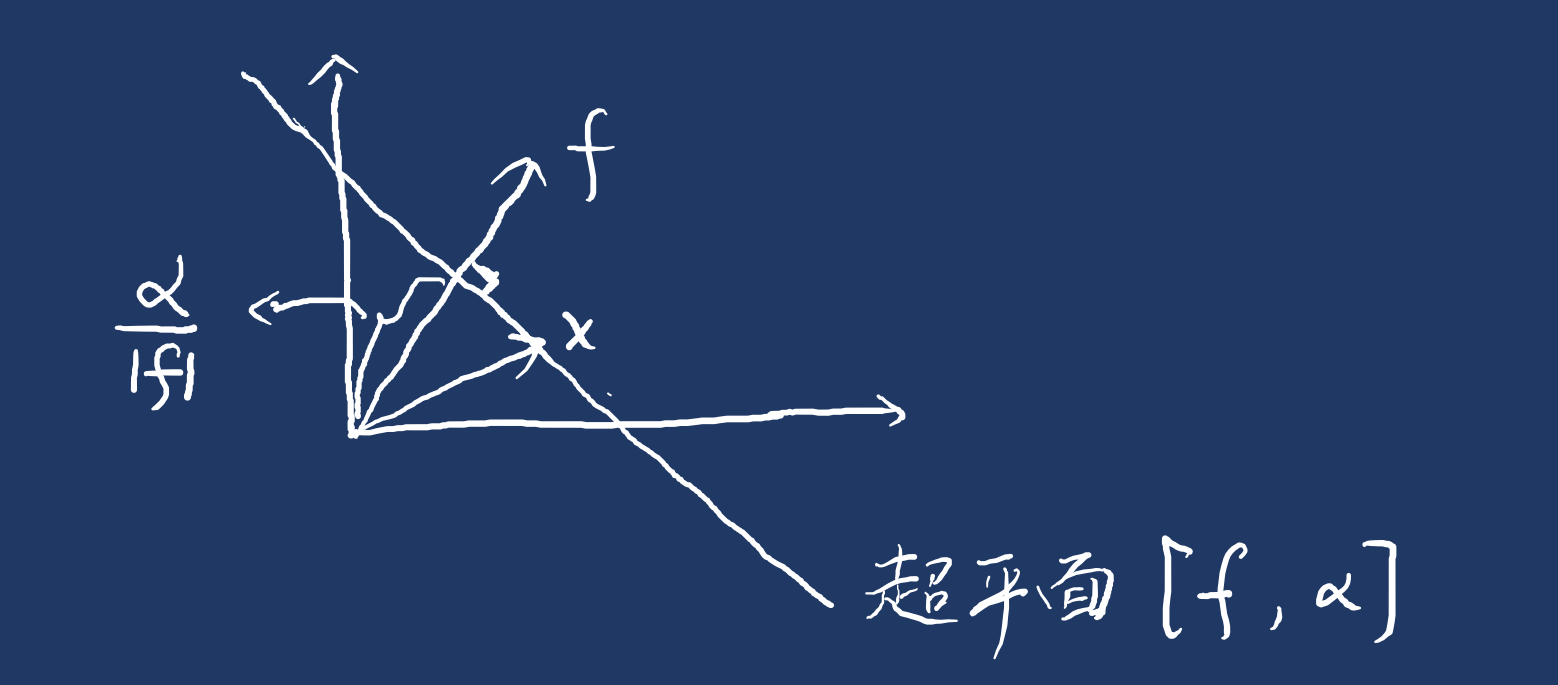
\includegraphics[width=0.5\textwidth]{figures/超平面.jpeg} % 替换为你的图片文件名
\end{figure}
\begin{definition}[凸集]
    点集 $C\st \RR^n$ 称为凸集,如果 $\forall x,y\in C$
    \[
    \lambda x+(1-\lambda)y\in C,\quad \forall \lambda\in [0,1]
    \]
\end{definition}

\begin{definition}[凸集严格分离]
    称凸集 $A,B$ 能被超平面 $[f,\alpha]$ 严格分离,如果
    \[
    \forall x\in A,f\cdot x\leq \alpha\quad \text{且}\quad \forall y\in B,f\cdot y>\alpha
    \]
    或
    \[
    \forall x\in A,f\cdot x< \alpha\quad \text{且}\quad \forall y\in B,f\cdot y\geq \alpha
    \]
    总之, $f\cdot y>f\cdot x,\forall x\in A,y\in B$
\end{definition}

\begin{figure}[H]
    \centering
    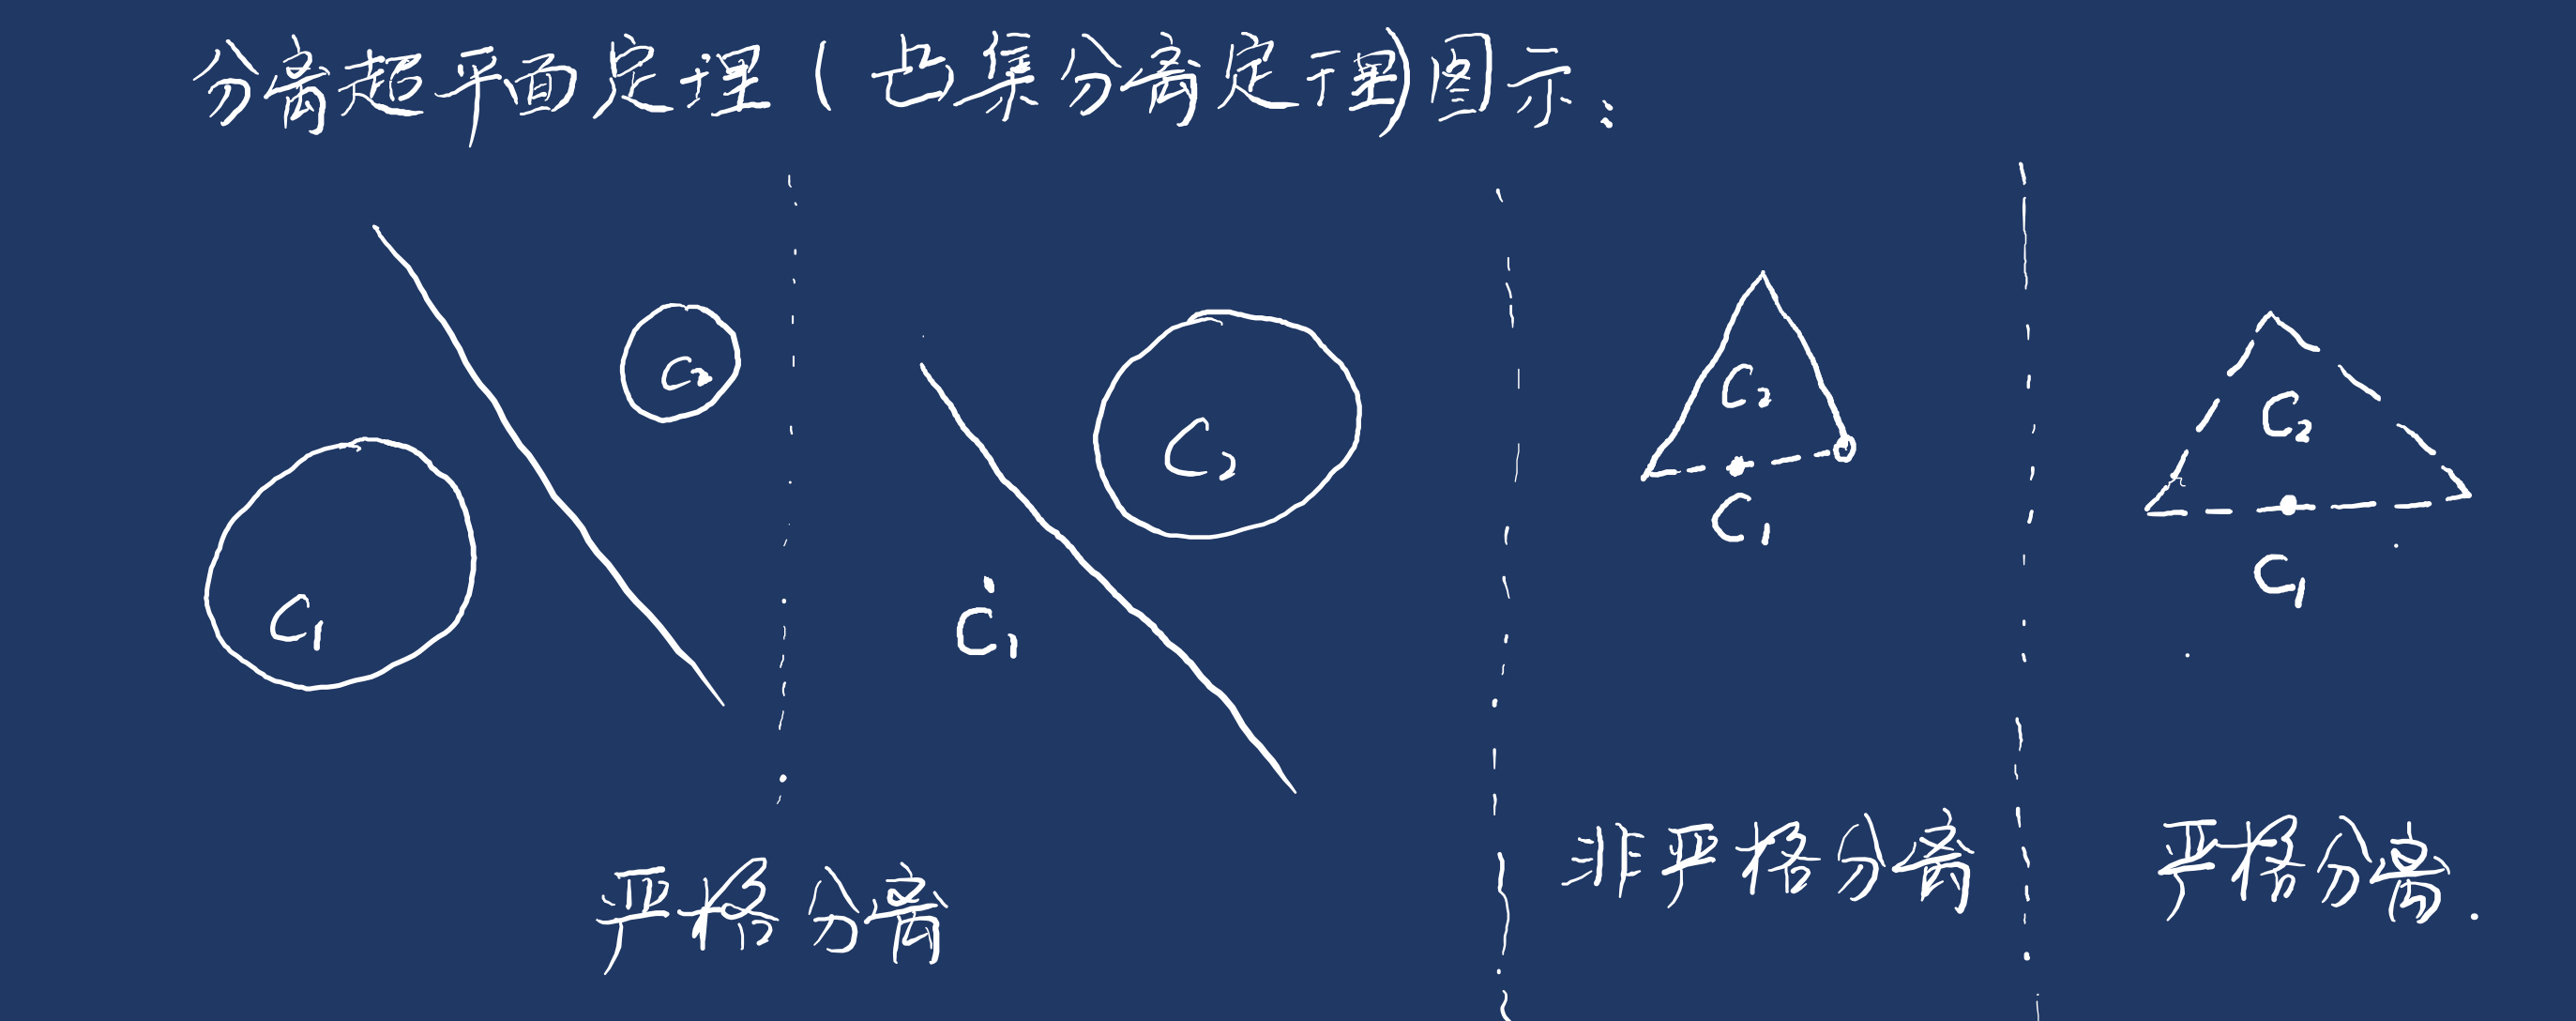
\includegraphics[width=0.8\textwidth]{figures/凸集分离.jpeg} % 替换为你的图片文件名
\end{figure}

\begin{definition}[点集的线性支撑集]
    点集 $C$ 的线性支撑集为
    \[
    C^l=\{\lambda x+(1-\lambda)y|\forall x,y\in C,\lambda \in \RR\}
    \]
\end{definition}

\begin{definition}[代数开集]
    点集 $C$ 称为是代数开集,如果 $C$ 为 $C^l$ 内的开子集(即 $C$ 为 $C^l$ 内的相对开集)
\end{definition}

\begin{example}
    设 $x_1,\cdots,x_K\in \RR^K$,令
    \[
    A=\{\sum_{i=1}^K\lambda_i x_i|\sum_{i=1}^K\lambda_i=1,\lambda_1\geq 0,\forall i=1,2,\cdots ,K\}
    \]
    \[
    B=\{\sum_{i=1}^K\lambda_i x_i|\sum_{i=1}^K\lambda_i=1,\lambda_1> 0,\forall i=1,2,\cdots ,K\}
    \]
    则 $A$ 为闭凸集,$B$ 为代数开凸集
\end{example}

\begin{theorem}[凸集分离定理]
    若 $C$ 为闭凸集或代数开凸集,且 $0\notin C$,则 $\{0\}$ 与 $A$ 被一个超平面严格分离,即存在 $f$ 使得
    \[
    f\cdot x>0,\quad \forall x\in A
    \]
\end{theorem}

\begin{theorem}
    在单时段模型中,不存在套利机会当且仅当存在风险中性概率测度 $\QQ$
\end{theorem}

证明:(1) $\Leftarrow$ 充分性

设风险中性测度 $\QQ$ 存在,即存在概率测度行向量 $\Pi>0$,使得 $\Pi(\Delta S^*)=0$,故 $\forall \hat{h}=(h_1,h_2,\cdots,h_m)^T$
\[
\Pi[(\Delta S^*)\hat{h}]=[\Pi(\Delta S^*)]\hat{h}=0
\]
于是不存在 $\hat{h}$,使得 $(\Delta S^*)\hat{h}\geq 0$,且不等号对某个 $\omega$ 严格成立

(2) $\Rightarrow$ 必要性

令 $P^+=\{\Pi|\Pi=(q_1,\cdots,q_K),\sum_{i=1}^Kq_i=1,q_i>0,\forall i=1,2,\cdots,K\}$,定义
\[
W=\{\Pi(\Delta S^*)|\Pi\in P^+\}
\]
则 $W$ 为代数开凸集

用反证法。若风险中性测度不存在,则 $0\notin W$,于是由凸集分离定理,存在向量 $\hat{h}=(h_1,\cdots,h_m)^T$,使得
\[
\Pi[(\Delta S^*)\hat{h}]=[\Pi(\Delta S^*)]\cdot \hat{h}>0,\quad \forall \Pi\in P^+
\]
故 $(\Delta S^*)\hat{h}\geq 0$ 且对某个 $\omega$ 不等号严格成立,因此套利交易策略存在,矛盾

\subsubsection{未定权益的可达性}

期权等衍生品在到期时刻的收益是样本空间 $\Omega$ 上的一个随机变量。一般地,$\Omega$ 上的任意随机变量 $Y$ 可以视作一个未定权益。

\begin{definition}[未定权益]
    未定权益(Contingent Claim)指的是在未来某一时刻(通常是到期时刻)的收益依赖于某些不确定因素的金融资产或合约。这些不确定因素通常与市场中的随机变量相关,比如股票价格、利率、汇率等。
\end{definition}

\begin{definition}[可达性]
    在单时段模型中,$t=1$ 时刻的未定权益 $Y$ 被称为是可达的,如果存在一个交易策略,使得
    \[
    Y(\omega)=V_1(\omega),\forall \omega\in \Omega
    \]
    也就是说,未定权益 $Y$ 可以由该交易策略下的投资组合复制,故由无套利性,未定权益 $Y$ 在 $t=0$ 时刻的价格为 $V_0$
\end{definition}

\begin{theorem}
    可达未定权益 $Y$ 在 $t=0$ 时刻的价格应为
    \[
    V_0=\EE_Q\left[\frac{Y}{1+r}\right]=\frac{1}{1+r}\EE_Q(Y)
    \]
\end{theorem}

风险中性概率测度的计算
\[
\begin{aligned}
    &\hat{S}^*(0)=\Pi\hat{S}^*(1;\Omega)\\
    &\Leftrightarrow \begin{cases}
        \sum_{i=1}^K q_i=1\\
        \Pi(\Delta S^*)=0
    \end{cases}
\end{aligned}
\]
其中 $\Pi=(q_1,q_2,\cdots,q_K)>0$

\begin{example}\label{exa:three-assets}
    若
    \[
    \hat{S}^*(1;\Omega)=\begin{pmatrix}
        1&4&3\\
        1&3&2\\
        1&2&4
    \end{pmatrix},\quad 
    \hat{S}^*(0)=(1,3,3)
    \]
    则风险中性测度满足
    \[
    \begin{cases}
        q_1+q_2+q_3=1\\
        4q_1+3q_2+2q_3=3\\
        3q_1+2q_2+4q_3=3
    \end{cases}\quad\Rightarrow\quad
    \begin{cases}
        q_1+q_2+q_3=1\\
        q_1-q_3=0\\
        -q_2+q_3=0
    \end{cases}
    \]
    解得 $\Pi=(1/3,1/3,1/3)$
\end{example}

\begin{example}\label{exa:two-assets}
    设
    \[
    \hat{S}^*(1;\Omega)=\begin{pmatrix}
        1 & 4\\ 1&3\\1&2
    \end{pmatrix},\quad \hat{S}^*(0)=(1,3)
    \]
    则风险中性测度满足
    \[
    \begin{cases}
        q_1+q_2+q_3=1\\
        4q_1+3q_2+2q_3
    \end{cases} \quad \Rightarrow \quad 
    \begin{cases}
        q_1+q_2+q_3=1\\
        q_1-q_3=0
    \end{cases}
    \]
    解得 $\Pi=(\lambda,1-2\lambda,\lambda)$,其中 $0<\lambda<\frac{1}{2}$
\end{example}

未定权益 $Y$ 可达当且仅当线性方程组 $\hat{S}^*(1;\Omega) \hat{h}=\overrightarrow{Y}^*$ 有解,其中 $Y^*=Y/(1+r)$
\[
\begin{aligned}
    \overrightarrow{Y}^*&=(Y^*(\omega_1), Y^*(\omega_2), \cdots, Y^*(\omega_K))^T\\
    \hat{h}&=(h_0,h_1,\cdots,h_M)^T
\end{aligned}
\]
或者说,未定权益贴现向量 $\overrightarrow{Y}^*$ 可以由所有已知证券的贴现价格向量 $S^*_0(1), S^*_1(1), S^*_2(1),\cdots,S^*_M(1)$ 线性表出,其中 $S_m^*(1)$ 为向量\eqref{eq:discount_vector}在 $t=1$ 时刻的取值。

若任意未定权益可达,则称该证券模型为完全市场。易知证券模型为完全市场的充要条件为矩阵 $\hat{S}^*(1;\Omega)$ 为行满秩的。

\begin{example}
    在例\ref{exa:two-assets}的模型中,贴现未定权益 $(5,4,3)^T$ 可达,而贴现未定权益 $(2,4,3)^T$ 是不可达的

    由风险中性定价原理知,贴现未定权益 $(5,4,3)^T$ 在 $t=0$ 时刻的价格应为
    \[
    5\lambda+4(1-2\lambda)+3\lambda=4
    \]
    而例\ref{exa:three-assets}的模型为完全市场,贴现未定权益 $(2,4,3)^T$ 在 $t=0$ 时刻的价格为
    \[
    2\times \frac{1}{3}+4\times \frac{1}{3}+3\times \frac{1}{3}=3
    \]
\end{example}

在例\ref{exa:two-assets}中,
\[
\hat{S}^*(1;\Omega)=\begin{pmatrix}
    1&4\\1&3\\1&2
\end{pmatrix},\quad \hat{S}^*(0)=\begin{pmatrix}
    1&3
\end{pmatrix},\quad \overrightarrow{Y}^*=(5,4,3)^T
\]
存在等价关系
\[
\begin{aligned}
    &\text{rank}(\hat{S}^*(1;\Omega);\overrightarrow{Y}^*)=\text{rank}(\hat{S}^*(1;\Omega))\\
    \Leftrightarrow& \overrightarrow{Y}^* \text{可由} \hat{S}^*(1;\Omega) \text{的列向量线性表示}\\
    \Leftrightarrow& \text{未定权益} Y \text{可达}
\end{aligned}
\]
\[
\begin{pmatrix}
    1&4&5\\
    1&3&4\\
    1&2&3
\end{pmatrix}\to \begin{pmatrix}
    1&4&5\\
    0&-1&-1\\
    0&-2&-2
\end{pmatrix}\to \begin{pmatrix}
    1&4&5\\
    0&-1&-1\\
    0&0&0
\end{pmatrix}
\]
因此 $\text{rank}(\hat{S}^*(1;\Omega);\overrightarrow{Y}^*)=\text{rank}(\hat{S}^*(1;\Omega))$,$Y$ 可达

$(\lambda,1-2\lambda,\lambda)$ 为风险中性概率
\[
\begin{pmatrix}
    1&4&2\\
    1&3&4\\
    1&2&3
\end{pmatrix}\to \begin{pmatrix}
    0&2&-1\\
    0&1&1\\
    1&2&3
\end{pmatrix}\to \begin{pmatrix}
    0&0&3\\
    0&1&1\\
    1&2&3
\end{pmatrix}
\]
$3=\text{rank}(\hat{S}^*(1;\Omega);\overrightarrow{Y}^*)\neq\text{rank}(\hat{S}^*(1;\Omega))=2$,$Y$ 不可达

\subsection{二期二叉树模型}

设第1期和第2期银行存款利分别为 $r_1,r_2$,求到期敲定价格为 $K$ 的欧式看涨期权的价格

股票价格二叉树:

\vspace{1em}

\begin{center}
    \begin{forest}
        for tree={grow'=east, l sep=30pt, s sep=15pt, inner sep=2pt}
        [{$a$}
            [{$b_1$}
                [{$c_1$}]
                [{$c_2$}]
            ]
            [{$b_2$}
                [{$c_3$}]
                [{$c_4$}]
            ]
        ]
    \end{forest}
\end{center}

\vspace{1em}

期权价格二叉树:

\vspace{1em}

\begin{center}
    \begin{forest}
        for tree={grow'=east, l sep=30pt, s sep=15pt, inner sep=2pt}
        [{$x$}
            [{$y_1$}
                [{$z_1=(c_1-K)^+$}]
                [{$z_2=(c_2-K)^+$}]
            ]
            [{$y_2$}
                [{$z_3=(c_3-K)^+$}]
                [{$z_4=(c_4-K)^+$}]
            ]
        ]
    \end{forest}
\end{center}

\vspace{1em}

计算股票二叉树的风险中性概率,故得

\vspace{1em}

\begin{center}
    \begin{forest}
        for tree={grow'=east, l sep=30pt, s sep=15pt, inner sep=2pt}
        [{$a$}
            [{$b_1$}, edge label={node[midway,above]{$q_1$}}
                [{$c_1$}, edge label={node[midway,above]{$q_2$}}]
                [{$c_2$}, edge label={node[midway,below]{$1-q_2$}}]
            ]
            [{$b_2$}, edge label={node[midway,below]{$1-q_1$}}
                [{$c_3$}, edge label={node[midway,above]{$q_3$}}]
                [{$c_4$}, edge label={node[midway,below]{$1-q_3$}}]
            ]
        ]
    \end{forest}
\end{center}

\[
\begin{aligned}
    y_1&=(1+r_2)^{-1}(q_2z_1+(1-q_2)z_2)\\
    y_2&=(1+r_2)^{-1}(q_3z_3+(1-q_3)z_4)\\
    x&=(1+r_1)^{-1}(q_1y_1+(1-q_1)y_2)
\end{aligned}
\]
整理期权价格公式得
\[
\begin{aligned}
    x&=(1+r_1)^{-1}(1+r_2)^{-1}[q_1q_2z_1+q_1(1-q_2)z_2+(1-q_1)q_3z_3+(1-q_1)(1-q_3)z_4]\\
    &=(1+r_1)^{-1}(1+r_2)^{-1}\EE_Q[(S_2-K)^+]
\end{aligned}
\]
其中 $\QQ(\omega_1)=q_1q_2,\QQ(\omega)=q_1(1-q_2),\QQ(\omega_3)=(1-q_1)q_3,\QQ(\omega_4)=(1-q_1)(1-q_3)$

考虑风险中性概率下的股票二叉树,设风险中性测度为 $\QQ$

\vspace{1em}
\begin{minipage}{0.5\textwidth}
    \begin{figure}[H]
        \centering
        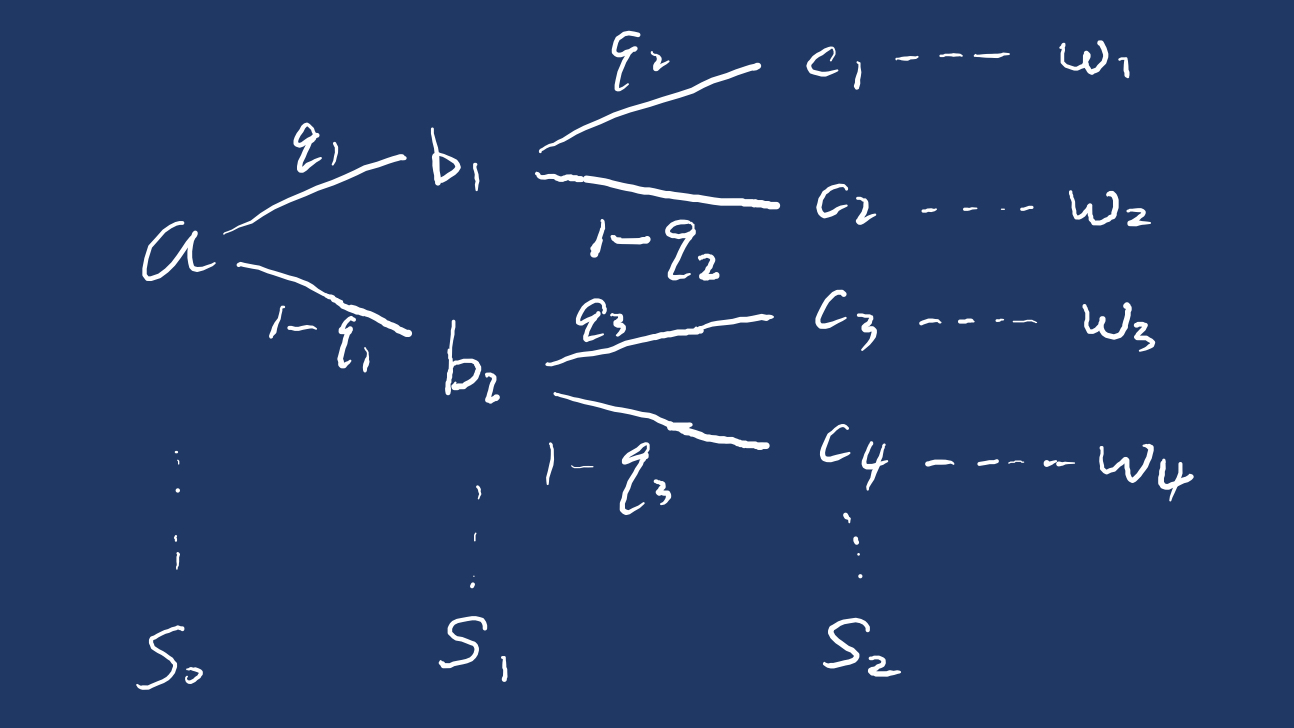
\includegraphics[width=\textwidth]{figures/二期二叉树.jpeg} % 替换为你的图片文件名
    \end{figure}
\end{minipage}
\begin{minipage}{0.5\textwidth}
    \[
    \begin{aligned}
        &\QQ\{S_1=b_1|S_0=a\}=q_1\\
        &\QQ\{S_1=b_2|S_0=a\}=1-q_1\\
        &\QQ\{S_2=c_1|S_0=a,S_1=b_1\}=q_2\\
        &\QQ\{S_2=c_2|S_0=a,S_1=b_1\}=1-q_2\\
        &\QQ\{S_2=c_3|S_0=a,S_1=b_2\}=q_3\\
        &\QQ\{S_2=c_4|S_0=a,S_1=b_2\}=1-q_3\\
    \end{aligned}
    \]
\end{minipage}
所以
\[
\begin{aligned}
    \QQ\{\omega_1\}&=\QQ\{S_0=a,S_1=b_1,S_2=c_1\}\\
    &=\QQ\{S_0=a\}\cdot \QQ\{S_1=b_1|S_0=a\}\cdot \QQ\{S_2=c_1|S_0=a,S_1=b\}\\
    &=q_1q_2
\end{aligned}
\]
同理
\[
\begin{aligned}
    &\QQ\{\omega_2\}=q_1(1-q_2)\\
    &\QQ\{\omega_3\}=(1-q_1)q_3\\
    &\QQ\{\omega_4\}=(1-q_1)(1-q_3)
\end{aligned}
\]
在风险中性概率测度 $\QQ$ 下,
\[
\begin{aligned}
    &\EE[S_1|S_0=a]=(1+r_1)a\\
    &\EE[S_2|S_0=a,S_1=b_1]=(1+r_2)b_1\\
    &\EE[S_2|S_0=a,S_1=b_2]=(1+r_2)b_2
\end{aligned}
\]
或者说
\[
\EE[S_1|S_0]=(1+r_1)S_0,\EE[S_2|S_0,S_1]=(1+r_2)S_1
\]
令 $S_2^*=(1+r_1)^{-1}(1+r_2)^{-1}S_2,S_1^*=(1+r_1)^{-1}S_1,S_0^*=S_0$,则
\[
\EE[S_1^*|S_0^*]=(1+r_1)^{-1}\EE[S_1|S_0]=S_0=S_0^*
\]
\[
\begin{aligned}
    \EE[S_2^*|S_0^*,S_1^*]&=(1+r_1)^{-1}(1+r_2)^{-1}\EE[S_2|S_0,S_1]\\
    &=(1+r_1)^{-1}S_1\\
    &=S_1^*
\end{aligned}
\]
换言之 $\{S_t^*,t=0,1,2\}$ 是一个 $Q$ 鞅

\subsubsection{信息结构和域流}

某风险资产的价格变化图

\begin{figure}[H]
    \centering
    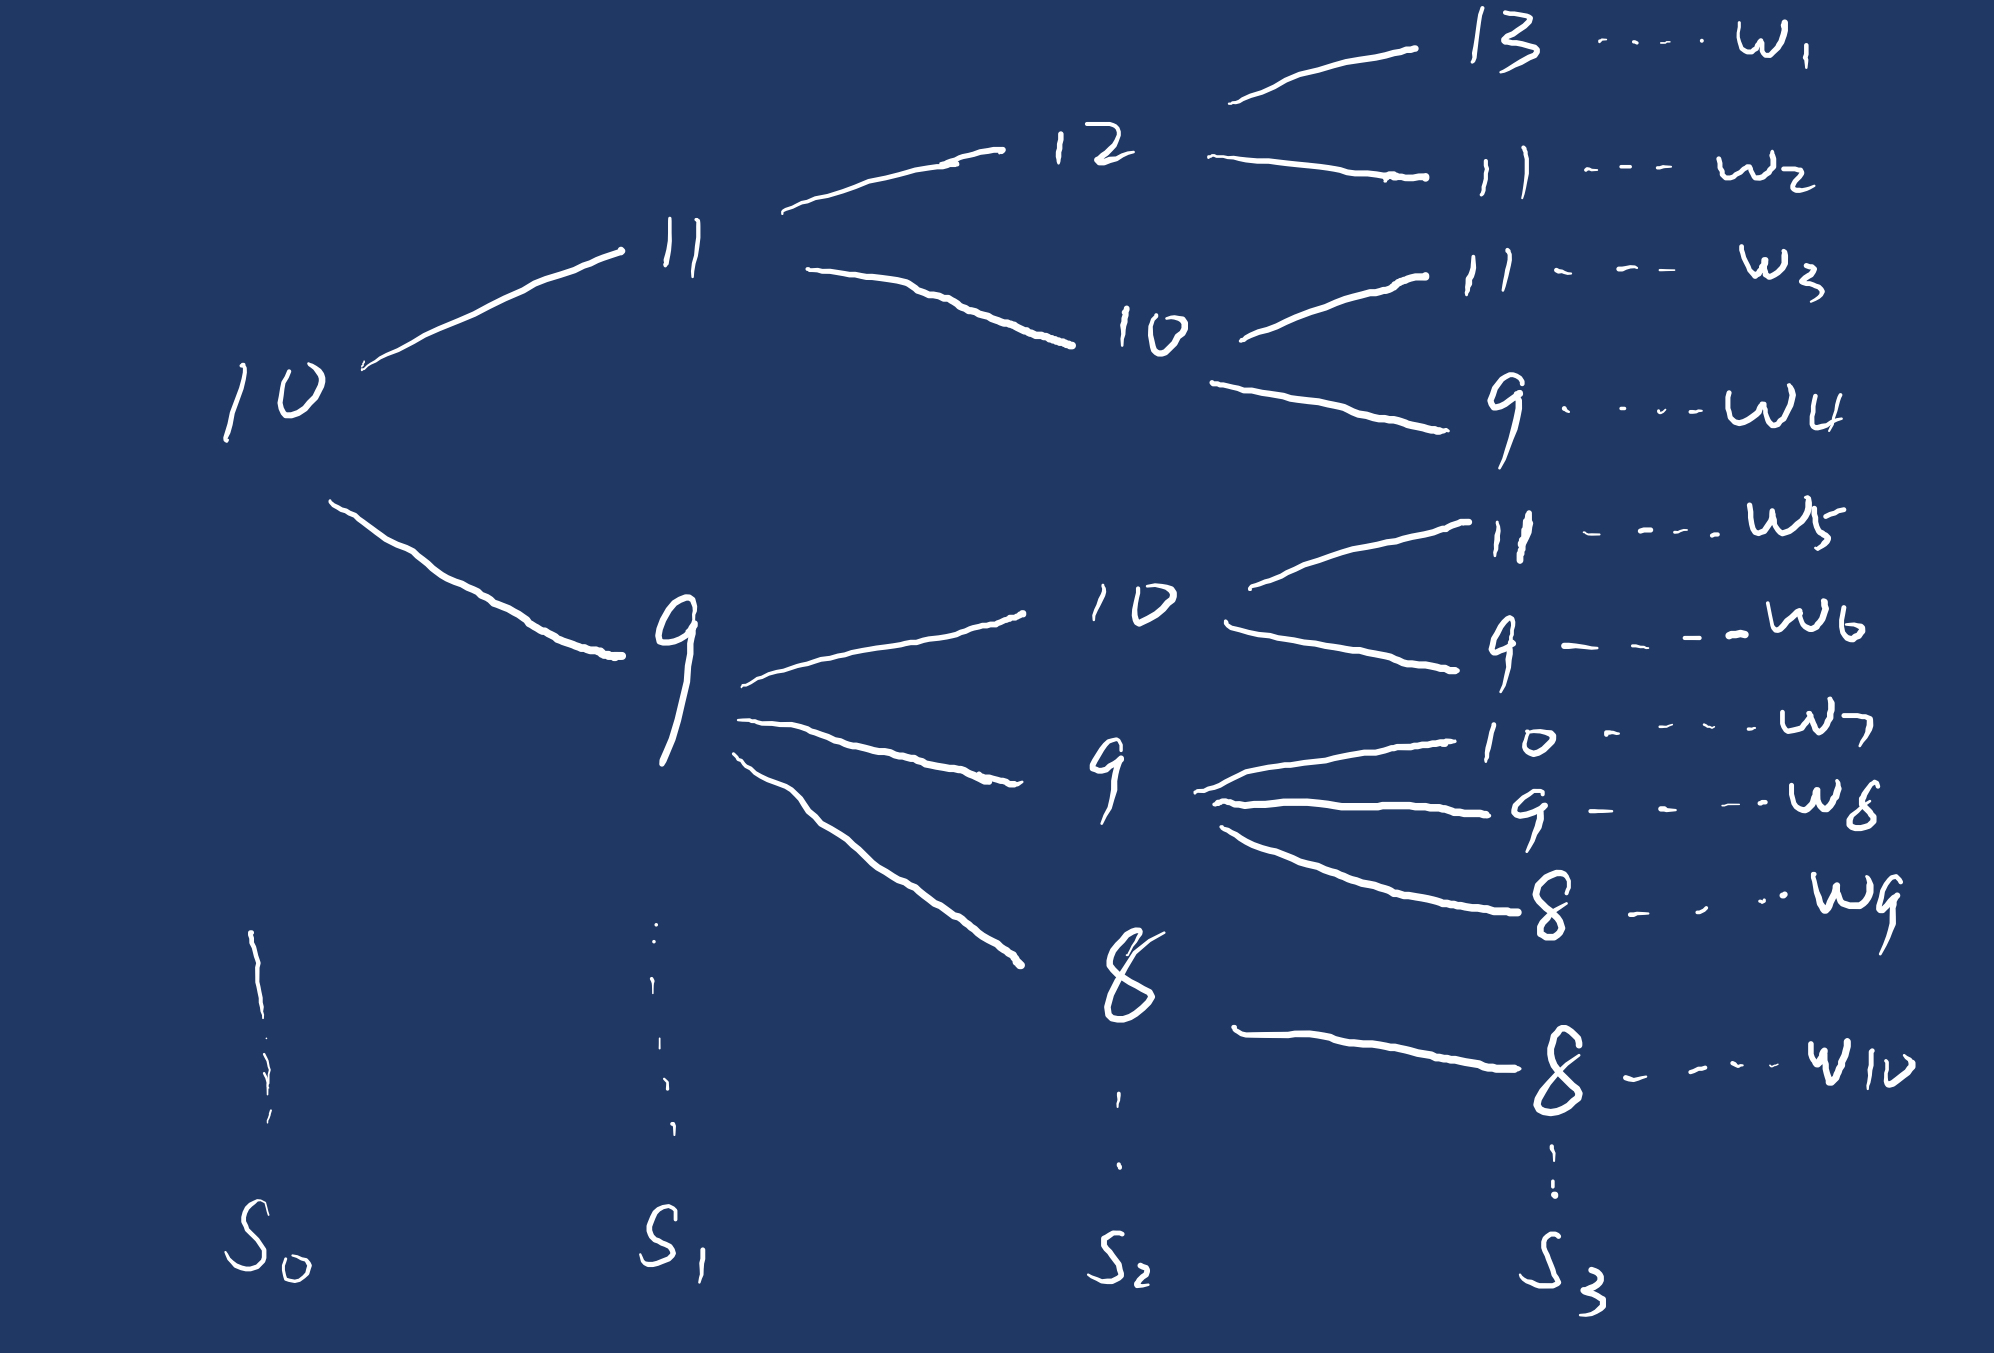
\includegraphics[width=0.7\textwidth]{figures/某风险资产价格变化图.jpeg} % 替换为你的图片文件名
    \label{fig:asset-price-chg}
\end{figure}

\begin{align*}
    \{ S_0 = 10 \} &= J_C = \{ \omega_1, \omega_2, \ldots, \omega_{10} \} \\
    \{ S_0 = 10, S_1 = 11 \} &= \{ \omega_1, \omega_2, \ldots, \omega_4 \} \\
    \{ S_0 = 10, S_1 = 9 \} &= \{ \omega_5, \omega_6, \omega_7, \omega_8, \omega_9, \omega_{10} \} \\
    \{ S_0 = 10, S_1 = 11, S_2 = 12 \} &= \{ \omega_1, \omega_2 \} \\
    \{ S_0 = 10, S_1 = 11, S_2 = 10 \} &= \{ \omega_3, \omega_4 \} \\
    \{ S_0 = 10, S_1 = 11, S_2 = 12, S_3 = 13 \} &= \{ \omega_1 \}
\end{align*}

信息树图

\begin{figure}[H]
    \centering
    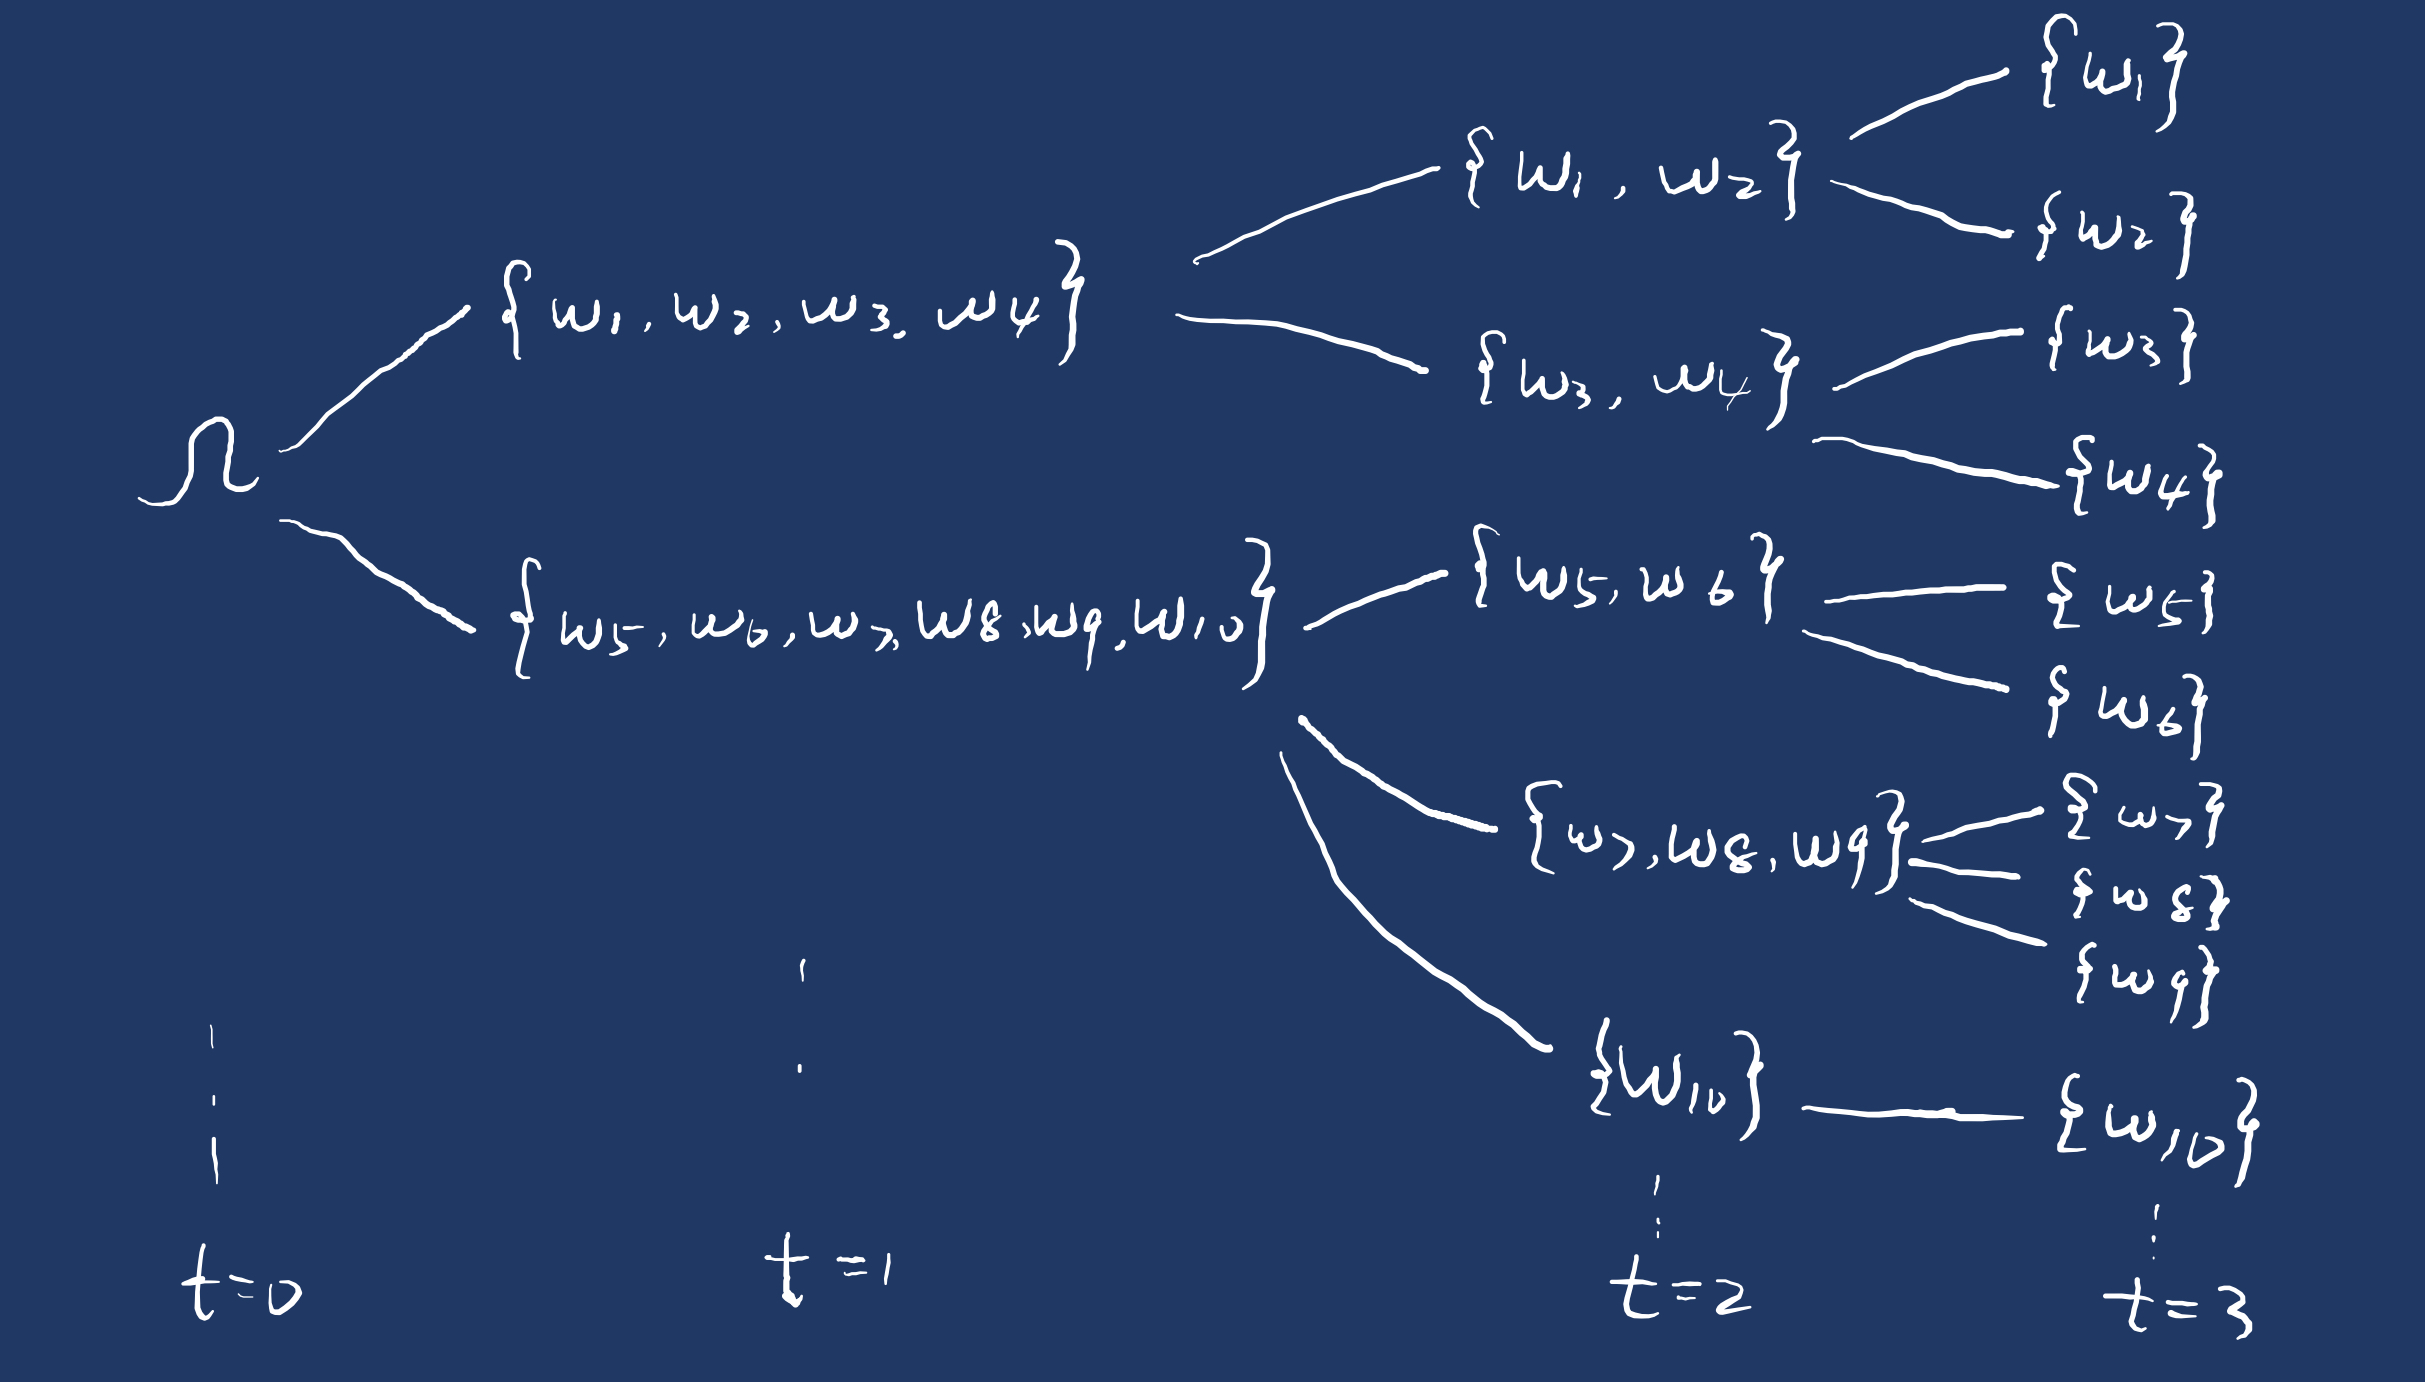
\includegraphics[width=0.7\textwidth]{figures/信息树图.jpeg} % 替换为你的图片文件名
\end{figure}

在各时刻所得到的信息可表示如下:

\begin{align*}
    p_0 &= \big\{ \{\Omega\} \big\} \\[8pt]
    p_1 &= \big\{ \{\omega_1, \omega_2, \omega_3, \omega_4\},\ \{\omega_5, \omega_6, \omega_7, \omega_8, \omega_9, \omega_{10}\} \big\} \\[8pt]
    p_2 &= \big\{ \{f\omega_1, \omega_2\},\ \{\omega_3, \omega_4\},\ \{\omega_5, \omega_6\},\ \{\omega_7, \omega_8, \omega_9\},\ \{\omega_{10}\} \big\} \\[8pt]
    p_3 &= \big\{ \{f\omega_1\},\ \{\omega_2\},\ \{\omega_3\},\ \{\omega_4\},\ \{\omega_5\},\ \{\omega_6\},\ \{\omega_7\},\ \{\omega_8\},\ \{\omega_9\},\ \{\omega_{10}\} \big\}
\end{align*}

上述 $p_0,p_1,p_2,p_3$ 对样本空间 $\Omega$ 的划分越来越精细,反映了随着时间的发展,所得到的信息越来越丰富

\begin{definition}[$\sigma$-代数]
    设 $\CF$ 是样本空间 $\Omega$ 中的一些子集构成的集合。称 $\CF$ 为一个 $\sigma$-代数,如果
    \begin{enumerate}
        \item $\Omega\in \CF$
        \item $B\in \CF\Rightarrow B^c\in\CF$
        \item $B_1,B_2,\cdots,B_n,\cdots\in \CF\Rightarrow \bigcup_{n=1}^{\infty}B_n\in \CF$
    \end{enumerate}
\end{definition}

设 $\mathcal{H}$ 为 $\Omega$ 的子集族(未必是 $\sigma$-代数),则必存在包含 $\mc{H}$ 的最小 $\sigma$-代数,称为由 $\mc{H}$ 生产的 $\sigma$-代数

\begin{example}
    设子集族 $\mc{H}=\{B_1,B_2,\cdots,B_n\}$ 是样本空间 $\Omega$ 的一个划分,则
    \[
    \sigma(\mc{H})=\{\bigcup_{j=1}^k B_{ij}|i_1,i_2,\cdots,i_k=1,2,\cdots,n;k=1,2,\cdots,n\}\cup \{\emp\}
    \]
\end{example}

回到前面的资产价格信息结构(图\ref{fig:asset-price-chg}),记
\[
\CF_i=\sigma\{p_i\},i=0,1,2,3
\]
则 $\CF_0\st \CF_1\st \CF_2\st \CF_3$,成为一个域流

\begin{definition}[域流]
    设 $\CF_t,t=0,1,\cdots,T$,均为样本空间 $\Omega$ 的 $\sigma$-代数,且 $\CF_0\st \CF_1\st \cdots\st \CF_T$,则称 $\{\CF_t,t=0,1,\cdots,T\}$ 为样本空间 $\Omega$ 的一个域流
\end{definition}

\begin{definition}[可测性]
    设 $\CF$ 为一个$\sigma$-代数,称任意随机变量 $X$ 关于 $\CF$ 可测,如果
    \[
    \{X\leq x\}\in \CF,\forall x\in \RR\tag{$*$}
    \]
    若 $X$ 为一个离散型r.v.,则$(*)$式等价于
    \[
        \{X= x\}\in \CF,\forall x\in \RR
    \]
\end{definition}

可测性表明, $X$ 的取值信息包含在 $\CF$ 中,换句话说 $\CF$ 的信息决定了 $X$ 的取值

\begin{property}
若 $X_1,\cdots,X_n$ 均关于 $\CF$ 可测,则 $g(X_1,\cdots,X_n)$ 也关于 $\CF$ 可测
\end{property}

\begin{property}
    若 $X_1,X_2,\cdots,X_n$ 均关于 $\CF$ 可测,则 $g(X_1,X_2,\cdots,X_n)$ 也关于 $\CF$ 可测
\end{property}

\subsubsection{随机变量的生成$\sigma$-代数}

若$\sigma$-代数$\CF$是使得随机变量$X_1,\cdots,X_n$可测的最小$\sigma$-代数,即
\[
\CF=\sigma\{X_1\leq t_1,\cdots ,X_n\leq t_n,\forall t_1,\cdots,t_n\in \RR\}
\]
记为
\[
\CF\overset{\Delta}{=}\sigma(X_1,\cdots,X_n)
\]

\begin{definition}[适应域流]
    如果对每个 $t=0,1,\cdots,T$,随机变量 $S(t)$ 都是 $\CF_t$ 可测的,则称随机过程 $\{S(t),t=0,1,\cdots,T\}$ 适应域流 $\{\CF_t,t=0,1,\cdots,T\}$,或称是关于 $\{\CF_t\}$ 的适应随机过程
\end{definition}

\begin{definition}[自然域流]
    若 $\CF_t=\sigma(S(0),S(1),\cdots,S(t))$,则称 $\{\CF_t,t=0,1,\cdots,T\}$ 为 $\{S(t)\}$ 的自然域流,它是使得 $\{S(t)\}$ 适应的最小域流
\end{definition}